\capitulo{3}{Conceptos teóricos}


\section{Fundamentos Básicos}

\subsection{La eficiencia}

La eficiencia vista desde un ámbito general se definiría como el uso racional de los recursos para conseguir un objetivo. Esta definición puede ser aplicada a cualquier ámbito en el que se hable de eficiencia pero en el caso de este proyecto se aplicará esta definición en el ámbito computacional.
La definición citada anteriormente menciona la palabra recursos, en el ámbito que estamos tratando, cuando se habla de recursos la palabra que más suele asociarse es tiempo. Esto no quiere decir que sea la única medida de eficiencia, ni mucho menos, también se podría poner como recurso el espacio en memoria, pero el tiempo suele ser el recurso que más condiciona y la gente más en cuenta tiene en las características de los  programas.\\

Aquí llegamos a la razón de existir de este proyecto, ¿cómo medimos lo que tarda un programa en ejecutarse de manera fiable?. La manera más extendida para hacer esto, es ejecutar el programa que se desee y esperar a que termine, contado el tiempo pasado desde el comienzo hasta el final de este. Esta manera a pesar de ser sencilla, a la hora de la verdad es muy poco fiable. Para que los resultados obtenidos por este método sean considerados verídicos se tendría que asegurar que el entorno de pruebas tenga unas condiciones idóneas, como por ejemplo que el procesador que del ordenador donde se ejecuta el programa no este gastando recursos en otros procesos que estén activos en segundo plano. El problema de esto es que conseguir un entorno así muchas veces no es tarea fácil. Y como respuesta a este problema surge la idea principal de este proyecto, medir la eficiencia de un programa de una manera fiable, que no se vea afectado por factores externos a este.\\

Para lograr un método para medir la eficiencia de un programa sin que su valor se vea afectado por el cuándo y dónde se haga el análisis, se decidió hacerlo a través de la identificación y el conteo operaciones que se ejecutan en el código del programa. Tras esto una vez se obtengan estas operaciones, se hará una ponderación a cada tipo de operación según el nivel de complejidad que se declare. 

\subsection{El intérprete}

Un intérprete es un programa que analiza y ejecuta el código de otro programa instrucción a instrucción. Esta es la manera con la que se pueden detectar los diferentes elementos que componen un programa. Al realizar este trabajo en Python hay que comentar antes que el interprete se trata de una máquina de pila\cite{MaquinaP}, lo que no deja de ser una máquina virtual que emula el funcionamiento de un ordenador. El funcionamiento principal de este se basa en almacenar y gestionar información que va recogiendo en las diversas pilas que tiene, para de esta manera poder hacer sus operaciones.\\

El interprete elegido para este trabajo se trata de ByteRun\cite{ByteRun}, un interprete hecho en código python y para código python. Este fue elegido por ser un interprete que fue creado con el objetivo principal el aprendizaje, lo cual conlleva que su complejidad no sea muy alta y por lo tanto es relativamente fácil implementar nuevas funcionalidades en este. Por otro lado en contra parte de esa baja complejidad hay que mencionar que ByteRun no es un intérprete muy rápido, como por ejemplo podría ser Cpython, pero como en este trabajo el principal requisito que se busca en un interprete es el de poder implementar nuevas funcionalidades en este para conseguir una forma de poder detectar las operaciones ejecutadas y guardarlas. ByteRun era una opción muy acertada que se adaptaba perfectamente a los requisitos del desarrollo.


\subsection{Bytecode}
ByteRun al ser un interprete de Python, no analiza directamente el código de alto nivel, lo que este analiza es un código intermedio llamado Bytecode.\\ El ByteCode es un código intermedio sacado a través de la traducción de un código de alto nivel al ser tratado por una serie de procesos (lexer,compiller...). Para sacar este código intermedio se ha utilizado un modulo de Python que actúa de desensamblador y descompone el código de alto nivel. 




\section{De código a Tiempo Computacional}

Una vez explicados los conceptos anteriores se para a contar los pasos llevados a cabo para conseguir traducir el código de alto nivel a una medida con la que se pueda medir la eficiencia,  el cual en el caso de este trabajo se ha optado por los ciclos de reloj.\\
Los pasos para hacer la transformación son los siguientes:\\
\begin{enumerate}
	\item Transformar el código de alto nivel a ByteCode a través del compilador.
	\item Traducir y ejecutar el ByteCode a través del intérprete.
	\item Obtener el diccionario de operaciones, mientras el interprete ejecuta el ByteCode.
	\item Ponderar los valores recogidos en el diccionario de operaciones con los procesadores teóricos para obtener el tiempo computacional.
\end{enumerate}

\imagen{Pasos}{Diagrama de flujo de la transformación del código de alto nivel al tiempo computacional}

\subsection{1º Paso: Obtención del ByteCode}.

Como ya se ha  comentado antes el ByteCode se trata  de un código intermedio sacado  a partir de la intervención de un compilador, para conseguir esto se cuenta con un modulo de Python llamado Dis que hace esta labor de compilador.\\
De primeras el aspecto de este código se trata de una serie de bytes que a simple vista una persona no podría entender.\\


\begin{figure}[H]
\centering
\begin{BVerbatim}
x=10
y=8
z=x*y
\end{BVerbatim}
\caption{Ejemplo de un código de alto nivel}
\end{figure}

Pero el modulo Dis, cuenta con una función que permite ver el ByteCode en una especie de lenguaje ensamblador, lo cual resulta muy útil para entender la estructura del código.\\

\begin{figure}[H]
\centering
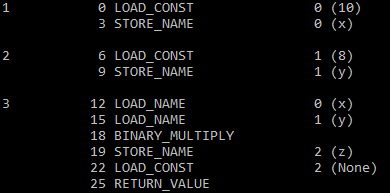
\includegraphics[width=8cm, height=5cm]{ByteCode}
\caption{Ejemplo del ByteCode en vista de ensamblador}
\end{figure}

La forma de entender este tipo de código es la siguiente:\\

Como ejemplo usaremos la primera fila donde se encuentra la instrucción ''LOAD CONTS'', la primera columna muestra el número 1 que representa la línea donde está la instrucción en el código de Python, la segunda columna es un índice que indica que la instrucción ''LOAD CONTS'', en En este caso, está en la posición 0, la tercera columna es el nombre de la instrucción en sí misma, mostrándola con un nombre comprensible para una persona, la cuarta columna indica la posición de ese argumento en la pila y la última columna muestra cuál es el argumento para la instrucción.\\

\subsection{2º Paso: Obtención del ByteCode}
Una vez obtenido el Bytecode entra en acción el interprete, en nuestro caso el ByteRun, el cual es capaz de ir analizando y ejecutando el bytecode obtenido.

\subsection{3º Paso: Matriz de operaciones}
El ByteRun no es capaz ir almacenando las operaciones que va traduciendo. En este momento es donde se debe implementar una nueva funcionalidad en el intérprete para que sea capaz de hacer esto, para así mas tarde poder hacer un cálculo de la eficiencia 

Cuando el ByteRun lee una instrucción y lo primero que tiene que hacer es identificar que tipo de instrucción esta leyendo, hay muchos tipos diferentes desde un ''LOAD'', a un ''LOOP'', o un ''ADD'', pero a nosotros no nos interesan todas las instrucciones, solo queremos almacenar aquellas que son consideradas por nosotros como ''operaciones'', o lo que es lo mismo, instrucciones que necesiten de algún tipo de calculo por parte del procesador, y que por lo tanto tenga un tiempo de ejecución.\\

Por suerte para nosotros el interprete ya hace distinciones entre los diferentes tipos de instrucciones y guarda en una lista todos aquellos valores en los cuales requiere hacer una operación.\\

Aprovechando esto, cada vez que alguna de esas instrucciones es llamada guardamos el nombre que tiene esta al ser visualizado el bytecode mediante el modulo dis\cite{dis} en una matriz, el cual decidimos llamar matriz de operaciones.\\

Esta matiz tiene la siguiente estructura:\\

\begin{table}[H]
\begin{center}
\begin{tabular}{|l|l|l|l|l|l|}
\hline
Operación & Operador & INT & STR & FLOAT & BOOL \\
\hline \hline
ADD & int & 1001 & 0 & 200 & 0\\ \hline
ADD & flo & 2004 & 0 & 2450 & 0 \\ \hline
MULTIPLY & int & 0 & 70 & 0 & 0 \\ \hline
MULTIPLY & flo & 0 & 0 & 555 & 0 \\ \hline
DIVIDE & int & 600 & 0 & 30 & 0 \\ \hline
\end{tabular}
\caption{Ejemplo de la estructura básica de la Matriz de operaciones.}
\label{tabla:sencilla}
\end{center}
\end{table}

La estructura de la matriz se basa en el hecho de que un operación necesita de dos valores con los que operar, y dependiendo del tipo de estos valores, dos mismas operaciones con diferentes valores, pueden llegar a tener nivel de eficiencia mucho mas bajo o alto que el otro. \\

Como se ve en la tabla 3.1, las dos primeras columnas de la matriz hacen de índice para las tuplas, la primera columna guarda el tipo de operación mientras que la segunda guarda el tipo del primer operador. Y la primera tupla de la matriz hace de indice para las columnas guardando los tipos del segundo operador, para así poder determinar la celda exacta donde se lleva la cuenta de una operación concreta.

Según el ByteRun va analizando todo el código cuando detecta una instrucción dentro de la lista de operaciones este llama a una función, la cual busca la posición celda correspondiente a la operación encontrada, una vez hallada incrementa en 1 el valor que se encuentre en la celda.\\

De esta manera cuando el ByteRun acaba de analizar todas las operaciones, conseguimos tener una matriz con el registro total de operaciones que han surgido a lo largo de la ejecución del programa.\\

\subsection{4º Paso: Ponderación}
Pero con solo tener los tipos de operaciones no es suficiente. Para hacer un análisis de la eficiencia es necesario saber el nivel de eficiencia que dispone cada tipo de operación, ya que no todas las operaciones tiene la misma complejidad y el procesador necesita hacer mas cálculos para ejecutarlos. Esto se consigue gracias al procesador teórico.\\

\subsubsection{Procesadores Teóricos}
El procesador teórico tiene la función de darle un nivel de eficiencia a cada tipo de operación. Se le puso este nombre por ser la parte que simula la complejidad que le supondría a un determinado procesador, de esta manera según los valores que se guarden en el procesador se pueden simular diferentes tipos de entornos.\\

Estos procesadores se tratan de unos ficheros de tipo .csv que guardan una matriz, llamada matriz de traducción. Esta matriz tiene una estructura pensada para poder almacenar los diferentes niveles de eficiencia que se les quiere asignar a cada operación en cada celda según se desee.\\

Sigue la misma estructura que la matriz de operaciones. Las dos primeras celdas de la matriz hacen de índice para las tuplas, la primera columna guarda el tipo de operación mientras que la segunda guarda el tipo del primer operador. Siguiendo esta estructura si tuviéramos por ejemplo una suma de un entero con un decimal, para encontrar el nivel de eficiencia que habría que aplicarle a esta operación en concreto la herramienta busca primero el tipo del operador, en este caso seria ''ADD'' y seguido a  esto busca en la segunda columna deja el valor ''int'', una vez  encontrados  estos dos valores ya tendría localizada la tupla donde se encuentra  el valor  deseado, y aquí es donde  entra en juego el indice de las  columnas que se haya en la primera fila de la matriz, esta  guarda los diferentes tipos que puede tomar el segundo operador, en este caso ''flo'', y con esto puede localizar que celda de la tupla es la que se necesita.

\begin{table}[H]
\begin{center}
\begin{tabular}{|l|l|l|l|l|l|}
\hline
Operación & Operador & INT & STR & FLOAT & BOOL \\
\hline \hline
ADD & int & 1 & 4 & 2 & 3\\ \hline
ADD & int & 2 & 2 & 2 & 2 \\ \hline
MULTIPLY & int & 1 & 2 & 3 & 2 \\ \hline
MULTIPLY & int & 1 & 4 & 2 & 2 \\ \hline
DIVIDE & int & 2 & 5 & 3 & 3 \\ \hline
\end{tabular}
\caption{Ejemplo de la estructura básica de la Matriz de traducción.}

\label{tabla:sencilla}
\end{center}
\end{table}



\subsubsection{Calculo de la Ponderación}
Una vez tenemos tanto la matriz de operaciones como un Procesador teórico ya solo falta realizar la ponderación para obtener los datos necesarios, en este caso los ciclos de reloj, para hacer los análisis oportunos. 

La formula aplicada para hacer la ponderación es la siguiente:

\begin{figure}[H]
\[
Tcloc=\sum_{i,j}^{(N,M)} M_{O}(i,j)M_{T}(i,j)
\]
\caption{Formula aplicada para hacer la ponderación.}
\end{figure}


Donde N y M son el número de filas y columnas de M O. Debe prestarse atención al tamaño de M T debe ser más grande que el tamaño de M O.
Aunque esta herramienta se ha desarrollado completamente en Python, y actualmente solo puede analizar archivos .py exclusivamente, una de las ideas principales es que luego se pueda usar en diferentes entornos, para diferentes tipos de lenguajes y pueda realizar una variedad más amplia de análisis, para así adaptarse mejor a las diferentes demandas que puede requerir el análisis en profundidad de la eficiencia de un código, en un entorno más exigente. Se decidió comenzar con este tipo de lenguaje, ya que Python hoy en día se usa ampliamente en diferentes campos como por ejemplo la robótica, gracias a la gran variedad de bibliotecas que tiene. Y sería muy interesante ver los resultados que se podrían obtener en todos estos campos.


\section{Tipos de Análisis}
Con los datos obtenidos ya se pueden hacer diferentes tipos de análisis, en el caso de esta herramienta se han implementado dos tipos:
\begin{itemize}
	\item Análisis individual
	\item Análisis comparativo
\end{itemize}
 

\subsection{Análisis Individual}
En este análisis solo se permite la entrada de un fichero,de formato .py, el cual tras pasar por los pasos citados en los puntos anteriores, muestra una gráfica circular con las diferentes operaciones que el interprete(ByteRun)a detectado al ejecutarlo. Y ademas de esto deja recalcular el resultado mostrado en el gráfico según las operaciones que queramos mostrar o no y el procesador con el que se quiera hacer la ponderación.\\

\imagen{Grafica1}{Gráfica resultante del análisis individual}


Este análisis esta pensado para optimizar el código del programa, ya que de esta manera puedes detectar que operaciones son las que mas recursos consumen.

\subsection{Análisis Múltiple}
En este análisis se eligen varios ficheros, los cuales son ejecutados y analizados para calcular los ciclos de reloj que tarda en ejecutarse cada uno. A la hora de mostrar los resultados puede variar la forma de represar la  información según el numero de ficheros que se hayan escogido. En caso de ser menos de 10 saldrá una gráfica de barras en la cual cada barra representa el total de ciclos de reloj de cada fichero. Y en caso de que se metan mas de 10 se cambiaría por una  gráfica de puntos para facilitar la visibilidad de los resultados. Al igual que en el análisis  individual en todo momento se pueden cambiar los resultados  de la gráfica cambiando las operaciones que queramos que se tengan en cuenta y el procesador  con el que se quiera ponderar las operaciones.\\

\begin{figure}[H]
\centering
\subfloat[Con menos de 10 ficheros]{
\label{f:Primero}
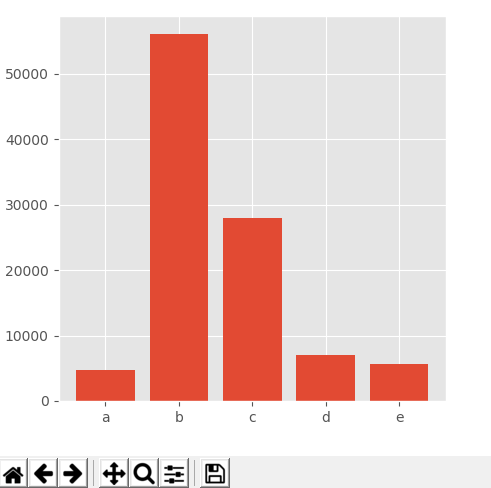
\includegraphics[width=7cm, height=5cm]{Grafica5}}
\subfloat[Con más de 10 ficheros]{
\label{f:Segundo}
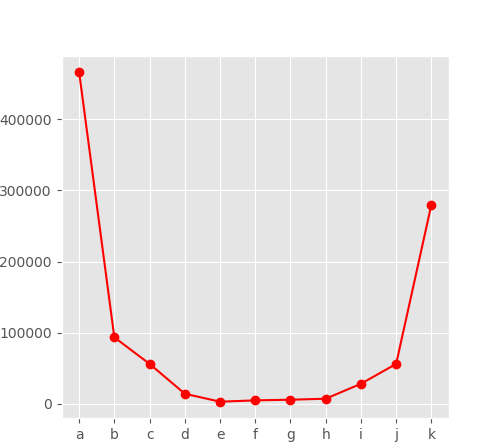
\includegraphics[width=7cm, height=5cm]{Grafica6}}
\caption{Gráficas resultantes del análisis múltiple}
\end{figure}


Este análisis esta pensado para compara ficheros que tengan como finalidad hacer lo mismo, y de esta manera saber cual de ellos tiene en que clase de entornos mejor eficiencia.


\section{Caso práctico de un Análisis}
Para entender mejor todos los conceptos teóricos a continuación se explicara un caso practico de un análisis múltiple.

En este análisis utilizaremos ficheros con el mismo código, pero a cada uno de estos se le cambiara algún parámetro, para así averiguar cual responde con mayor eficiencia. El código utilizado se muestra en la figura 3.6.

\begin{figure}[H]
\centering
\begin{BVerbatim}
tEnd=100; ts=0.1
KP=2; KD=8; KI=1
t=0; e=0; eSum=0; eOld=0
while t < tEnd:
	t=t+ts
	e=SIGNAL-REF
	OUT=KP*e + KD*(e-eOld)/ts + KI*eSum*ts
	eOld=e
	eSum+=e 
\end{BVerbatim}
\caption{Vista del código de alto nivel que se utiliza para hacer el análisis}
\end{figure}


Una vez seleccionados los archivos que queremos analizar, se llama al modulo dis para traducir los códigos a ByteCode (figura 3.8).\\
Cuando ya se ha logrado el ByteCode, es cuando el intérprete comienza a realizar sus funciones y genera el contenido de la matriz de operaciones (tabla 3.3).

\begin{table}[H]
\begin{center}
\begin{tabular}{|l|l|l|l|l|l|}
\hline
Operación & Operador & INT & STR & FLOAT & BOOL \\
\hline \hline
ADD & int & 2001 & 0 & 1002 & 0\\ \hline
ADD & int & 0 & 0 & 1001 & 0 \\ \hline
MULTIPLY & int & 3003 & 0 & 1001 & 0 \\ \hline
SUBTRARCT & int & 2002 & 0 & 0 & 0 \\ \hline
DIVIDE & int & 0 & 0 & 1001 & 0 \\ \hline
\end{tabular}
\caption{Ejemplo de la estructura básica de la Matriz de operaciones.}

\label{tabla:sencilla}
\end{center}
\end{table}

En la tabla anterior, una de las matrices de operación se ha mostrado de manera resumida, solo se muestran las tuplas que contienen algún valor. Cabe señalar que habría n Matrices, una para cada archivo analizado.

\begin{figure}[H]
\centering
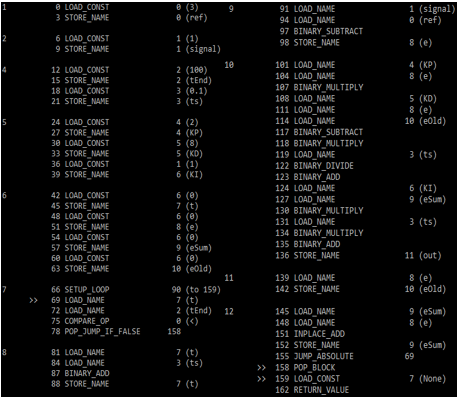
\includegraphics[width=10cm, height=9cm]{EjemploByte}
\caption{Vista del ByteRun resultante de uno de los ficheros}
\end{figure}

Después de calcular la matriz de operaciones, debemos elegir el procesador deseado para ponderar las operaciones contenidas en la matriz de operaciones. Aquí elegimos de acuerdo al campo en el que queremos que funcione el código. Y para eso tenemos que saber qué valores hay dentro de la matriz de traducción (tabla 3.4).

\begin{table}[H]
\begin{center}
\begin{tabular}{|l|l|l|l|l|l|}
\hline
Operación & Operador & INT & STR & FLOAT & BOOL \\
\hline \hline
ADD & int & 1 & 4 & 2 & 3 \\ \hline
ADD & int & 2 & 0 & 2 & 2 \\ \hline
MULTIPLY & int & 1 & 2 & 3 & 2 \\ \hline
SUBTRARCT & int & 1 & 4 & 2 & 2 \\ \hline
DIVIDE & int & 2 & 5 & 3 & 3 \\ \hline
\end{tabular}
\caption{Ejemplo de la estructura básica de la Matriz de traducción.}
\end{center}
\end{table}



Como en la vista de la matriz de operaciones, solo se muestran en esta vista las tuplas que tienen un valor relevante para el ejemplo que estamos ejecutando. En una vista total de la matriz de traducción hay muchas más filas.\\


Para verificar la validez de la técnica, la herramienta se ejecuta en un análisis de varios archivos, cada archivo tiene diferentes valores de tEnd y ts para el código de la figura 3.7. Los resultados se muestran en la tabla 3.5.\\

\begin{table}[H]
\begin{center}
\begin{tabular}{|l|l|l|l|}
\hline
File & tEnd & ts & Clock cycles \\
\hline \hline
A & 500 & 0.015 & 466676\\ \hline
B & 100 & 0.015 & 93338\\ \hline
C & 400 & 0.1 & 56000\\ \hline
D & 100 & 0.1 & 14014\\ \hline
E & 100 & 0.5 & 2800\\ \hline
F & 100 & 0.3 & 4676\\ \hline
G & 200 & 0.5 & 6000\\ \hline
H & 100 & 0.2 & 7000\\ \hline
I & 100 & 0.05 & 28014\\ \hline
J & 100 & 0.025 & 56000\\ \hline
K & 500 & 0.025 & 280014\\ \hline
\end{tabular}
\caption{Vista del valor de los parámetros de cada fichero con los ciclos de reloj resultantes.}
\end{center}
\end{table}


Con todos estos datos, la herramienta hace su análisis y nos muestra los resultados de la figura:

\begin{figure}[H]
\centering
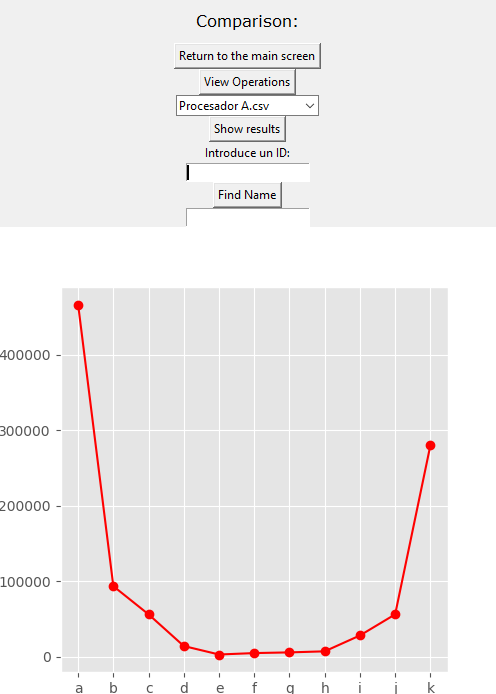
\includegraphics[width=8cm, height=10cm]{resultados}
\caption{Vista de los resultados del análisis de eficiencia}
\end{figure}

Como puede verse en la figura 3.9 y la tabla 3.5, los mejores resultados se obtienen con el archivo e, con los parámetros tEnd = 100 y ts = 0.5.